\documentclass[11pt]{article}
\usepackage{cite}
\usepackage{graphicx}

\begin{document}
\title{Kernel Density Estimation Writeup}
\date{Today}
\maketitle

\section{Kernel density estimation}
As shown in Fig. \ref{fig:perp_distribution} and Fig. \ref{fig:distribution}, the pattern of the photons occupancy on the PMT plane can be very complicated.  Consequently, fitting an analytic curve to the data was determined to be infeasible.  As an alternative fitting method, we are trying Kernel Density Estimation \cite{rosenblatt1956}.
\begin{figure}
\centering
\includegraphics[width=4in]{pngs/perp_distro.png}
\caption{Accumulated photon occupancy for an incoming pion perpendicular to the bars at 4.5 GeV.  This geometry has the segmented mirrors and water filling the readout box.\label{fig:perp_distribution}}
\end{figure}
\begin{figure}
\centering
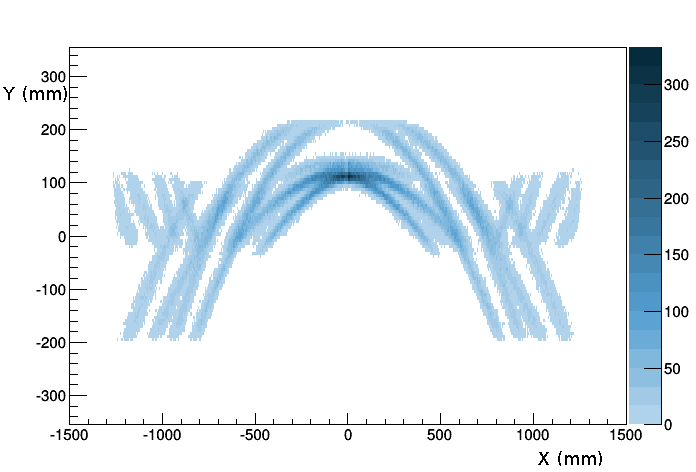
\includegraphics[width=4in]{pngs/fitdirc_ang440_3seg_index_5000MeV_133_pion_dist.png}
\caption{Accumulated photon occupancy for an incoming pion with $\theta=4^{\circ}$ and $\phi=40^{\circ}$ at 4.5 GeV.  This geometry has the segmented mirrors and water filling the readout box.\label{fig:distribution}}
\end{figure}
Kernel density estimation works by using a set of monte carlo points to produce an estimate of the Probability Distribution Function ("PDF") on the PMT plane.  The function is obtained by adding the value of a spreading function around each of the points used for estimation.  To do a proper estimation, this simulation used approximately $2*10^5$ of these points, which will be refered to hereafter as the "provisional" points.  This is in contrast to the (about) $25$ "real" points which would be detected from an actual charged particle passing through the bar.

While there are several possible options for spreading functions, such as a truncated parabola ("Epanechnikov") or a uniform distribution, for this analysis, a gaussian is chosen as the spreading function mostly due to its familiarity.  In the early stages of the analysis, several possible functions were tried and little variation was found between them.  

Explicitly, the probability at a point $\vec{x}$ (a 2d point on the PMT plane)  with a set of $N_p$ provisional points $\vec{p_i}$ is taken to be the normalized form of:

\begin{equation}
\textrm{pdf}(x) = \sum\limits_{i=1}^{N_p} \textrm{g}(\frac{|p_i-x|}{\lambda})
\end{equation}
with:
\begin{equation}
\textrm{g}(y) = \textrm{exp}(\frac{-y^2}{2})
\end{equation}
Where g is our gaussian spreading function and lambda is optimized based on the number of provisional points.  $\lambda$ is also known as the bandwidth, and scales non-trivially with $N_p$, so once an $N_p$ is chosen, several values of $\lambda$ are tried until the one with the best performance (as defined below) is found \cite{SJOS:SJOS445}.

\section{Using the PDFs}
Using the DiRC geometry, it is possible to simulate the path of a photon from its creation all the way onto the PMT plane. It is also possible to know within a certain precision the trajectory and energy of an incident particle using the information of the other sub-detectors.  Using the kinematic information to produce the correct distribution of photons, one hypothesis PDF for each candidate particle is created.  This is done by tracking the photons from their production to the plane and using Kernel Density Estimation to fill in the PDF.  In order to identify particles, we classify the candidate particles as the possible particle types that could have produced a hit in the DiRC.  Typically these will be pions, kaons, and sometimes protons, so 2-3 candidate pdfs are created per real hit in the DiRC.

In the following, the pion and the kaon were considered as candidate particles. The study was performed at 4.5 and 5 GeV/c to produce a measurable overlap.  

In order to do so, $N_x$ photons (representing the expected number of detected photons during the experiment) for each candidate particle were tracked during the simulation up to the PMT plane, and $N_p$ photons were generated to produce the PDFs of the 2 candidates.  These $N_x$ particles were then used to compute the loglikelihood from each candidate PDF.  The loglikelihoods were computed as follows:

\begin{equation}
ll_{pion} = \sum\limits_{j=1}^{N_x} \textrm{ln}(\sum\limits_{i=1}^{N^{pion}_{p}} \textrm{g}(\frac{|p^{pion}_{i}-x_j|}{\lambda}))
\end{equation}
and:
\begin{equation}
ll_{kaon} = \sum\limits_{j=1}^{N_x} \textrm{ln}(\sum\limits_{i=1}^{N^{kaon}_{p}} \textrm{g}(\frac{|p^{kaon}_{i}-x_j|}{\lambda}))
\end{equation}

$N_p$ is typically large and currently chosen such that the achieved resolution reaches a stable value.  $N_x$ is normalized to 25 for a perpendicular tracks according to the experimental data from SLAC.

The difference in these loglikelihoods is then reported as the figure of merit to cut on.  The histograms of the loglikelihood difference for a pion versus a kaon is shown in Fig. \ref{fig:llhistos}.

\begin{figure}
\centering
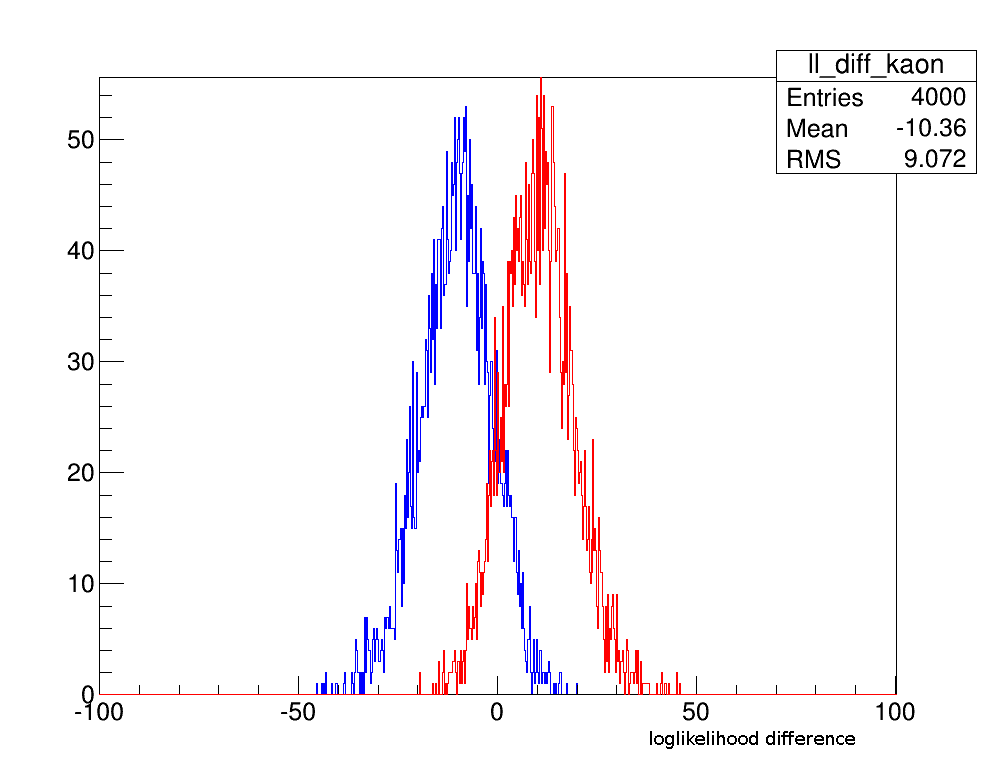
\includegraphics[width=4in]{pngs/ll_diffs.png}
\caption{$ll_{pion} - ll_{kaon}$ for a track at 5 GeV and $\theta=4^{\circ}$ and $\phi=40^{\circ}$.  The readout box is filled with water.  Pion values shown in red, while kaon values shown in blue. \label{fig:llhistos}}
\end{figure}

To quantify the performance, a ROC (Receiver Operating Characteristic) curve is produced as in Fig. \ref{fig:roccurve}.  The ROC curve is a way of reperesenting all possible loglikehood cuts on one plot.  It is defined parametrically with the parametric variable being the position on the $x$ axis of Fig. \ref{fig:llhistos}.  Then, the $x$ value of the ROC curve is the integral from the right to that position of the pion histogram, while the $y$ value is the integral from the left to that position of the kaon histogram.  In the plot, these are refered to as the pion efficiency ("Fraction of correctly identified pions with a lefted handed cut) and kaon missid (fraction of kaons identified as pions with a left handed cut) respectively.  A ROC curve of ideal separation has an area of 1 and is a perfect square, so areas under the curve are used to quantify the separating power of a given variable.  Note that this study assumes that there are an equal number of incoming pions and kaons.  If this is not the case, the the ROC curve will change shape.  The number of pions and kaons being equal is just to extract a resolution.

Then the integral of this ROC curve is compared to the integral of a ROC curve of two ideal gaussians with a mean separation equal to the nominal angular separation of the pion and kaon Cerenkov angles. That is, the cerenkov angles for a pion and a kaon in an $n = 1.47$ media are computed.  Subtracting these two angles gives the distance between the means of the gaussians.  The gaussians have the same standard deviation, and this standard deviation is set such that the integrals of the two ROC curves agree.  This value is then quoted as the nominal resolution.  In the example figure shown in Fig. \ref{fig:roccurve}, the integral is 0.956, which corresponds to a resolution of 1.74 mrad.
\begin{figure}
\centering
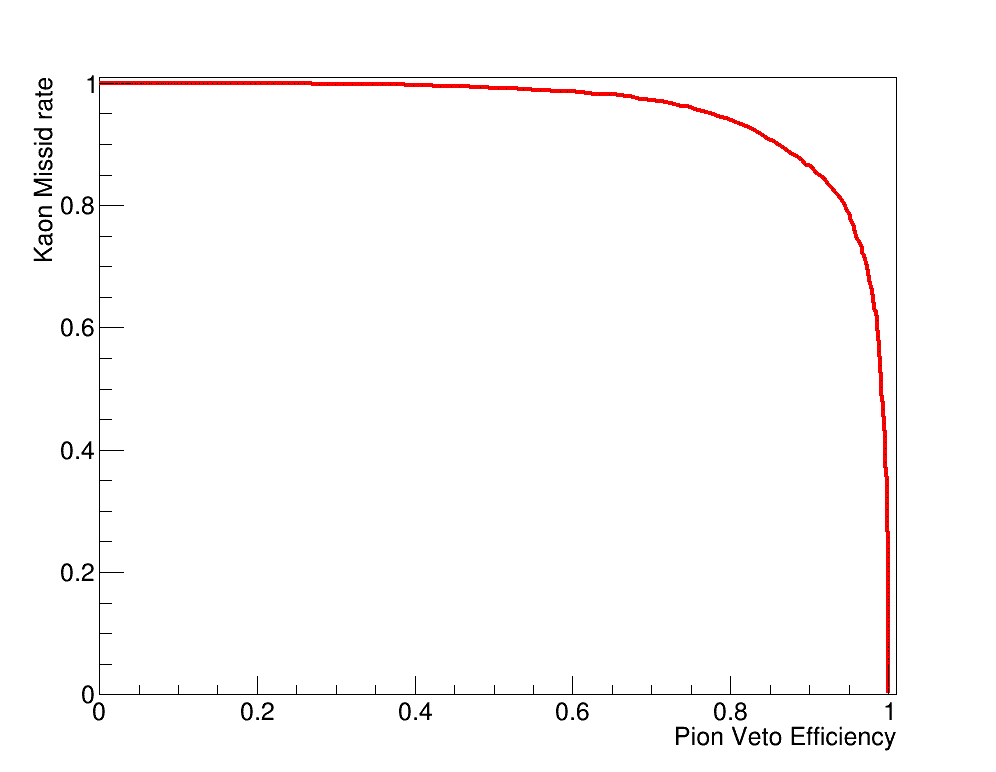
\includegraphics[width=4in]{pngs/roc_curve.png}
\caption{ROC curve for the histograms in Fig. \ref{fig:llhistos} \label{fig:roccurve}}
\end{figure}
\begin{figure}
\centering
\includegraphics[width=4in]{pngs/roc_over.png}
\caption{The same ROC curve as in Fig. \ref{fig:roccurve} (red) compared to a ROC curve for an 2 ideal gaussians with separation 4.05 mrad and standard deviation 1.74. \label{fig:roccurve_over}}
\end{figure}

The area under a ROC curve for two gaussians each with standard deviation $\sigma$ and means separated by $a$ can be obtained as follows:

\begin{equation}
\int_{-\infty}^{\infty} \textrm{GausCDF}(t,\sigma)*\textrm{Gaus}(t-a,\sigma)\,dt
\end{equation}

Using this integral, $\sigma$ is numerically solved for such that the integral is equal to that of the ROC curve generated to obtain the nominal resolution.  This resolution stays about the same when probed at different energies, and scales roughly with $\frac{1}{\sqrt{N_x}}$ as expected.

\section{Speed Considerations}
A major drawback of this method is that it requires a large number of points to accurately approximate the provisional PDF (the resolution plataeus at ~2e5). To that end, the simulation code must be written to allow a fast computation of the PDF.  Initially, the simulation was done entirely through GOptical \cite{goptical}, with the physics processes (PMTs quantum efficiency, surface effect, Cerenkov spectrum, transmittance etc.) being computed manually, but achieving a small reconstruction rate. The most significant performance drag is the number of reflections required to propagate the photons through the bars.  An analytical approach is now used to transport the photons to the end of the bars, avoiding the computation of the bounces during the propagation. The current reconstruction rate is currently about 1-10 Hz depending on the parameters chosen and shape of the PDF. But efforts will be made to optimize the code and it is expected to be able to reach a 50Hz reconstruction once the tracking is fully done by specialized c++ code (rather than letting GOptical handle the focusing mirrors as is done now).


\bibliography{bibliography}{}
\bibliographystyle{plain}
\end{document}